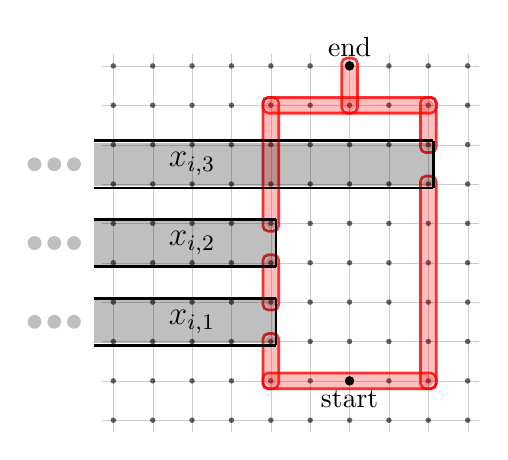
\begin{tikzpicture}[scale=0.50]
\def\wi{0.08}
\def\op{0.2}
\def\pts{2.0pt}
\foreach \x in {-6,...,3} {
\foreach \y in {-1,...,8} {
\fill[black, opacity=0.6] (\x, \y) circle (\pts);
}
}

\foreach \x in {-6,...,3} {
\draw[black, line width = \wi, opacity=\op] (\x, -1.3) -- (\x, 8.3);
}
\foreach \y in {-1,...,8} {
    \draw[black, line width = \wi, opacity=\op] (-6.3,  \y) -- (3.3, \y);

}
%\draw[red, line width = 2.267716536pt]   (-2, 0) -- (2, 0);
\draw[red, line width=1pt, opacity=0.8, rounded corners=2pt] (-2.2, -0.2) rectangle (2.2, 0.2);
\fill[red, opacity=0.25, rounded corners=5pt] (-2.2, -0.2) rectangle (2.2, 0.2);

%\draw[red, line width = 2.267716536pt]   (-2, 0) -- (-2, 1);

\draw[red, line width=1pt, opacity=0.8, rounded corners=2pt] (-2.2, -0.2) rectangle (-1.8, 1.2);
\fill[red, opacity=0.25, rounded corners=5pt] (-2.2, -0.2) rectangle (-1.8, 1.2);

% \draw[red, line width = 2.267716536pt]   (-2, 2) -- (-2, 3);

\draw[red, line width=1pt, opacity=0.8, rounded corners=2pt] (-2.2, 1.8) rectangle (-1.8, 3.2);
\fill[red, opacity=0.25, rounded corners=5pt] (-2.2, 1.8) rectangle (-1.8, 3.2);

% \draw[red, line width = 2.267716536pt]   (-2, 4) -- (-2, 7);


\draw[red, line width=1pt, opacity=0.8, rounded corners=2pt] (-2.2, 3.8) rectangle (-1.8, 7.2);
\fill[red, opacity=0.25, rounded corners=5pt] (-2.2, 3.8) rectangle (-1.8, 7.2);


% \draw[red, line width = 2.267716536pt]   (2, 0) -- (2, 5);


\draw[red, line width=1pt, opacity=0.8, rounded corners=2pt] (1.8, -0.2) rectangle (2.2, 5.2);
\fill[red, opacity=0.25, rounded corners=5pt] (1.8, -0.2) rectangle (2.2, 5.2);

%\draw[red, line width = 2.267716536pt]   (2, 6) -- (2, 7);


\draw[red, line width=1pt, opacity=0.8, rounded corners=2pt] (1.8, 5.8) rectangle (2.2, 7.2);
\fill[red, opacity=0.25, rounded corners=5pt] (1.8, 5.8) rectangle (2.2, 7.2);


%\draw[red, line width = 2.267716536pt]   (-2, 7) -- (2, 7);
\draw[red, line width=1pt, opacity=0.8, rounded corners=2pt] (-2.2, 6.8) rectangle (2.2, 7.2);
\fill[red, opacity=0.25, rounded corners=5pt] (-2.2, 6.8) rectangle (2.2, 7.2);

%\draw[red, line width = 2.267716536pt]   (0, 7) -- (0, 8);
\draw[red, line width=1pt, opacity=0.8, rounded corners=2pt] (-0.2, 6.8) rectangle (0.2, 8.2);
\fill[red, opacity=0.25, rounded corners=5pt] (-0.2, 6.8) rectangle (0.2, 8.2);

\filldraw (0, 0) circle (3pt);
\node[below] at (0, 0) {start};
\filldraw (0, 8) circle (3pt);
\node[above] at (0, 8) {end};
%\draw[red, line width=1pt, opacity=0.8, rounded corners=2pt] (-0.2, 6.8) rectangle (0.2, 8.2);
\draw[black, line width = 1pt]   (-6.5, 2.1) -- (-1.87, 2.1);
\draw[black, line width = 1pt]   (-6.5, 0.9) -- (-1.87, 0.9);
\draw[black, line width = 1pt]   (-1.87, 2.1) -- (-1.87, 0.9);
\draw[black, line width = 1pt]   (-6.5, 4.1) -- (-1.87, 4.1);
\draw[black, line width = 1pt]   (-6.5, 2.9) -- (-1.87, 2.9);
\draw[black, line width = 1pt]   (-1.87, 4.1) -- (-1.87, 2.9);
\draw[black, line width = 1pt]   (-6.5, 6.1) -- (2.13, 6.1);
\draw[black, line width = 1pt]   (-6.5, 4.9) -- (2.13, 4.9);
\draw[black, line width = 1pt]   (2.13, 6.1) -- (2.13, 4.9);
\draw[black, opacity=0.25, line width = 15.590551185000002pt]   (-6.5, 1.5) -- (-1.87, 1.5);
\draw[black, opacity=0.25, line width = 15.590551185000002pt]   (-6.5, 3.5) -- (-1.87, 3.5);
\draw[black, opacity=0.25, line width = 15.590551185000002pt]   (-6.5, 5.5) -- (2.13, 5.5);
\fill[black, opacity=0.25] (-7, 1.5) circle (5pt);
\fill[black, opacity=0.25] (-7.5, 1.5) circle (5pt);
\fill[black, opacity=0.25] (-8, 1.5) circle (5pt);
\node at (-4, 1.5) { \large $x_{i, 1}$};
\fill[black, opacity=0.25] (-7, 3.5) circle (5pt);
\fill[black, opacity=0.25] (-7.5, 3.5) circle (5pt);
\fill[black, opacity=0.25] (-8, 3.5) circle (5pt);
\node at (-4, 3.5) { \large $x_{i, 2}$};
\fill[black, opacity=0.25] (-7, 5.5) circle (5pt);
\fill[black, opacity=0.25] (-7.5, 5.5) circle (5pt);
\fill[black, opacity=0.25] (-8, 5.5) circle (5pt);
\node at (-4, 5.5) { \large $x_{i, 3}$};
\end{tikzpicture}
%[Finished in 0.2s]